
\begin{enumerate}
\item Selecteer de Grafische installatie interface in de Debian Installer Menu (\ref{DebInstallMenu}).

\begin{figure}[H]
	\centering
	\includegraphics[width=\linewidth]{debian_install_01.png}
	\caption{Debian Installer Menu}
	\label{DebInstallMenu}
\end{figure}

\item Selecteer daarna de Engelse taal. Bij problemen is de kans dat er iemand in het Engels het probleem al eens is tegengekomen vele malen groter dan in het Nederlands, dus wen je aan om in het Engels te werken met Linux.

\item Bij Location kiezen we eerst other en daarna Europe en dan Netherlands.

\item Voor de Locales laten we staan en\_US.UTF-8.

\item Voor de keyboard houden we American English aan, tenzij je een specifiek toetsenbord hebt.

\item De volgende keuze die je moet maken is die voor een hostname, kortom hoe gaat je computer heten. Kies hiervoor je achternaam met 01 eraan vast. Voor mij zou dat dus leeuw01 zijn. Let op! allemaal kleine letters.

\item De keuze voor het domein waarin de machine zit is lastig omdat we geen domein hebben. Het makkelijkst is om hier voorlopig localdomain in te vullen. We kunnen dat later nog wijzigen.

\item Nu moeten we een root wachtwoord kiezen. Het is verstandig om een sterk wachtwoord te kiezen, omdat de root gebruiker alles mag.

\item Ook voor de gebruiker is dat een goed plan. Gebruik een password manager om een wachtwoord te generen of om je gekozen wachtwoorden erin op te slaan.

\item We houden de harddisk indeling simpel, dus kiezen we Guided als onze optie voor de harddisk indeling zoals aangegeven in \ref{DebDiskPart}.

\begin{figure}[H]
	\centering
	\includegraphics[width=\linewidth]{debian_install_partition.png}
	\caption{Debian Disk Partitioning}
	\label{DebDiskPart}
\end{figure}

\item We kiezen de enige harddisk die er is en kiezen voor All files in one partition. In het overzicht dat we te zien krijgen zien we dat er naast een bestandssysteem ook een swap-partitie aangemaakt is zoals weergeven in figuur \ref{DebDiskParts}.

\begin{figure}[H]
	\centering
	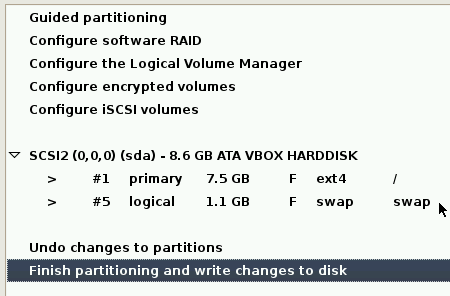
\includegraphics[width=\linewidth]{Debian_Install_Partitioned.png}
	\caption{Debian Disk Overview}
	\label{DebDiskParts}
\end{figure}

\item Nadat we hebben gekozen voor Yes bij de vraag of we het zeker weten zal Debian beginnen met de installatie van het systeem.

\item Na de installatie van het base system (een minimaal systeem), krijgen we de vraag of we nog meer software van andere CD's willen installeren. Dat willen we niet.

\item Debian gaat nu opzoek naar updates en additionele software die ge\"installeerd kan worden. De repo's van Debian staan over de wereld verspreid, om geen data op te halen van bijvoorbeeld servers in de Verenigde Staten, maar alleen van servers in Nederland, zodat de belasting van het Internet alleen lokaal is, moeten we een keuze maken vanaf welke servers wij onze software willen ophalen. Kies Netherlands en deb.debian.org. We gebruiken geen proxy dus bij die vraag mag je continue geven.

\item Debian gaat nu de databases ophalen van alle software die er voor Debian beschikbaar is en gaat daarna meteen je systeem updaten met de laatst beschikbare versies. Afhankelijk van hoe nieuw de ISO was waarvan je hebt geboot kan dit even duren. Je kan af en toe een vraag krijgen van de installer, lees de tekst dan goed en bepaal door en bepaal of je het wel of niet wilt wat er gevraagd wordt, of vraag je docent.

\item Als de update klaar is krijg je de keuze om nog extra software te installeren (zie \ref{DebSoft}).

\begin{figure}[H]
	\centering
	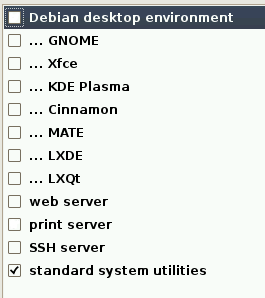
\includegraphics[width=\linewidth]{Debian_Install_Software_uit.png}
	\caption{Debian Additional Software Choice}
	\label{DebSoft}
\end{figure}

We willen alleen de Standard System Utilities, dus die moet aan. De rest moet uit staan.

\item Nadat Debian klaar is met de installatie kiezen we ervoor om GRUB te installeren in de master boot record

\item We selecteren \textbf{/dev/sda} (zie \ref{DebGrubDev}
\begin{figure}[H]
	\centering
	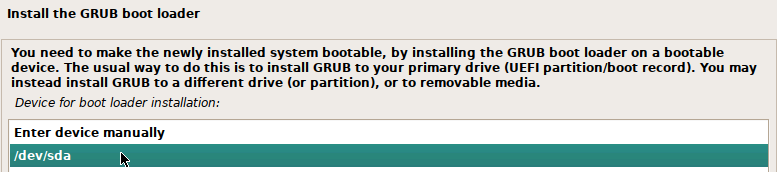
\includegraphics[width=\linewidth]{Debian_Install_Grub-device.png}
	\caption{Debian Install Grub Device}
	\label{DebGrubDev}
\end{figure}

\item Als alles klaar is rebooten we het systeem.
\end{enumerate}

Login als \texttt{root} met het root-wachtwoord dat je hebt aangemaakt tijdens de installatie. Installeer het sudo pakket:
\begin{lstlisting}[language=bash]
# apt-get install sudo
\end{lstlisting}

Voeg daarna jezelf als gebruiker toe aan de sudo groep:
\begin{lstlisting}[language=bash]
# usermod -a -G sudo dennis
\end{lstlisting}
Vervang \texttt{dennis} door je eigen gebruikersnaam; degene die je aangemaakt hebt bij de installatie.

We loggen uit:
\begin{lstlisting}[language=bash]
# exit
\end{lstlisting}

We loggen nu in als een gewone gebruiker. Nadat je ingelogd bent type je op de prompt:
\begin{lstlisting}[language=bash]
$ sudo shutdown -h now
\end{lstlisting}
Je VM zal afsluiten en uit gaan. Voortaan gebruik je altijd dit commando om je VM uit te zetten. Zet je VM nooit uit met de power-knop, het kan je Linux-systeem beschadigen en dan moet je deze hele installatie opnieuw doen.


